\documentclass[11pt,a4paper]{article}
\usepackage[utf8]{inputenc}
\usepackage[T1]{fontenc}
\usepackage[romanian]{babel}
\usepackage[margin=1.9cm]{geometry}
\usepackage{amsmath,amssymb}
\usepackage{enumitem}
\usepackage{parskip}
\usepackage{tikz}
\usetikzlibrary{arrows.meta,positioning,calc}
\setlist{nosep, topsep=2pt, itemsep=2pt, leftmargin=1.3em}
\setlength{\parskip}{3pt}
\pagestyle{empty}

\begin{document}
\begin{center}
{\small Universitatea Transilvania din Bra\c{s}ov}\\
{\small Departamentul de Automatic\u{a} \c{s}i Tehnologia Informa\c{t}iei}\\[4pt]
{\large\bfseries BILET DE EXAMEN}\\[1pt]
{\small sesiunea toamn\u{a} 2026}
\end{center}
\vspace{0.15cm}

\begin{enumerate}[leftmargin=1.4em]

\item Fie sistemul din figur\u{a} ($T_e=1$s):

\begin{center}
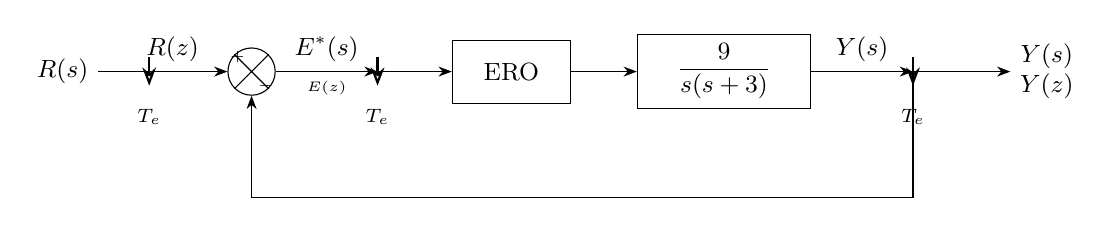
\begin{tikzpicture}[>=Stealth, font=\small]
\node (R) at (0,0) {$R(s)$};
\coordinate (swR) at (1.1,0);
\node[draw,circle,minimum size=6mm] (sum) at (2.4,0) {};
\draw (sum.north west) -- (sum.south east) (sum.north east) -- (sum.south west);
\node at ($(sum)+(-0.18,0.18)$) {\tiny$+$};
\node at ($(sum)+(0.18,-0.18)$) {\tiny$-$};

\coordinate (sw) at (4.0,0);
\node[draw,minimum width=15mm,minimum height=8mm] (ero) at (5.7,0) {ERO};
\node[draw,minimum width=22mm,minimum height=8mm] (g) at (8.4,0) {$\dfrac{9}{s(s+3)}$};
\coordinate (swY) at (10.8,0);
\node (Yout) at (12.5,0) {$\begin{matrix}Y(s)\\ Y(z)\end{matrix}$};

\draw[->] (R) -- (swR) node[midway,above]{} -- (sum) node[midway,above,pos=0.3]{$R(z)$};
\draw[-{Stealth[open]},thick] ($(swR)+(0,0.18)$) -- ++(0,-0.36);
\node[below] at ($(swR)+(0,-0.35)$) {\scriptsize $T_e$};
\draw[->] (sum) -- (sw) node[midway,above]{$E^*(s)$} node[midway,below]{\tiny$E(z)$};
\draw[-{Stealth[open]},thick] ($(sw)+(0,0.18)$) -- ++(0,-0.36);
\node[below] at ($(sw)+(0,-0.35)$) {\scriptsize $T_e$};
\draw[->] (sw) -- (ero);
\draw[->] (ero) -- (g);
\draw[->] (g) -- (swY) node[midway,above]{$Y(s)$};
\draw[-{Stealth[open]},thick] ($(swY)+(0,0.18)$) -- ++(0,-0.36);
\node[below] at ($(swY)+(0,-0.35)$) {\scriptsize $T_e$};
\draw[->] (swY) -- (Yout);

\draw[->] (swY) |- ++(0,-1.6) -| (sum);
\end{tikzpicture}
\end{center}

\begin{enumerate}[label=\alph*)]
\item S\u{a} se determine func\c{t}ia de transfer discret\u{a} a sistemului \^{i}n circuit \^{i}nchis. (1p)
\item Folosind ecua\c{t}ia cu diferen\c{t}e, s\u{a} se determine func\c{t}ia de transfer discret\u{a} a sistemului \^{i}n circuit deschis. (1p)
\item S\u{a} se determine pentru ce tip de intrare sistemul prezint\u{a} eroare sta\c{t}ionar\u{a} finit\u{a}. (0.5p)
\item S\u{a} se determine r\u{a}spunsul sistemului la m\u{a}rimea de intrare treapt\u{a} unitar\u{a} \c{s}i s\u{a} se reprezinte grafic. (1p)
\item S\u{a} se traseze caracteristicile de frecven\c{t}\u{a} amplitudine-pulsa\c{t}ie \c{s}i faz\u{a}-pulsa\c{t}ie. (1.5p)
\item S\u{a} se determine modelul cu variabile de stare pentru sistemul discret \^{i}n circuit \^{i}nchis. (1p)
\end{enumerate}
\emph{*pt punctele c,d,e,f se vor folosi rezultatele de la punctul a.}

\item Se consider\u{a} un sistem cu reac\c{t}ie negativ\u{a} unitar\u{a}, \^{i}n care func\c{t}ia de transfer a sistemului \^{i}n circuit deschis este de urm\u{a}toarea form\u{a} ($T_e=1$s):
$$G_d(z)=\frac{0.368\,k\,(z+0.717)}{z^2-1.368z+0.368}$$

Determina\c{t}i:
\begin{enumerate}[label=\alph*)]
\item Polii \c{s}i zerourile; nr. de ramuri ale locului r\u{a}d\u{a}cinilor; de unde \^{i}ncep ramurile \c{s}i unde se termin\u{a}. (0.2p)
\item Por\c{t}iunea de pe axa real\u{a} care apar\c{t}ine locului r\u{a}d\u{a}cinilor. (0.15p)
\item Nr. de asimptote, unghiul pe care-l fac cu axa real\u{a} \c{s}i punctul unde se \^{i}nt\^{a}lnesc pe axa real\u{a}. (0.15p)
\item Punctele de ramifica\c{t}ie. (0.5p)
\item Verifica\c{t}i dac\u{a} locul r\u{a}d\u{a}cinilor descrie un cerc. Trasa\c{t}i locul r\u{a}d\u{a}cinilor. (1p)
\end{enumerate}

\end{enumerate}

\textbf{Teorie:}
\begin{enumerate}[leftmargin=1.4em]
\item Transformarea planului $s$ \^{i}n planul $z$ (por\c{t}iunea 5-6).
\item Cu ce frecven\c{t}\u{a} trebuie e\c{s}antionat un semnal pentru a nu avea fenomenul de aliasing?
\item Care sunt etapele din procesul de conversie analog-numeric\u{a}?
\item S\u{a} se e\c{s}antioneze un semnal oarecare continuu. Reface\c{t}i semnalul continuu de la pasul anterior din e\c{s}antioanele sale, folosind ERO.
\end{enumerate}

\vspace{0.2cm}
\small Toate subiectele teoretice valoreaz\u{a} 1 punct.

\end{document}
